% The Models
\documentclass[../main]{subfiles}
\graphicspath{{figures/}{../figures/}}

\begin{document}
\subsection{Fast Response Model}
To discuss the possible deployment of drones in order to detect fire and transmit the signal to EOC,
 we design Fast Response Model to maximize coverage and minimize the cost. To represent the fire distribution,
  fire frequency and fire size, we come up with several well-designed indices and use fire location in certain
   period to represent those factors with minimum lost of information.  Since it's not economically
    efficient to cover all the land of Victoria because the drones are able to move and the fact that fire can
     spread and then be detected, we use weighted covering lost(WCL) to represent the cost for not covering 
     all the possible locations of fire. We use the data in 2020 for case study, but the strategy we adapt and
      the data we compute is generic and can be used in various situation. \\

      After sensitivity test, we proved the robustness of the model. It can be showed that the Fast Response Model can be used in different size of fire, different frequency of fire, and different distribution of fire in state of Victoria and other places in the world.
\subsubsection{Data Pre-processing}
For the sake of CFA, our model should only be considering the fire situation within the range of state of Victoria. The data we obtained from NASA database is contains noise and locations out of border. The first step of data pre-processing is meant to sift out all the illegal point with criteria mentioned above. Considering the spatial location of noise point,
 we use DBSCAN clustering with ball tree \cite{enwiki:1065597644} algorithm, and is implemented by sci-learn 
 project\cite{scikit-learn}. 
 Since the data contains latitude and longitude, 
 to define the distance function for clustering one need to use the haversine formula\cite{haversine} to calculate the great-circle distance between two points.
 
 \begin{equation}
      dist_{i,j}=2\cdot R_{e} \cdot \arctan \Bigg(\sqrt{\frac {\sin^2(\frac {\Delta \varphi_{lat} }{2})+\cos\varphi _i\cdot 
      \cos \varphi _j \cdot \sin^2({ \frac {\Delta \lambda_{lon}} {2} })}
      {1-(\sin^2(\frac {\Delta \varphi_{lat} }{2})+\cos\varphi _i\cdot 
      \cos \varphi _j \cdot \sin^2({ \frac {\Delta \lambda_{lon}} {2} }))}}\Bigg)
\end{equation}

This ensures the correctness of clustering.

To define a noise point which is inefficient to cover it, we define two
variables \(eps\) and \(minPoints\) according to DBSCAN conventions.

To more easily obtain the optimized value, we first normalize data with
standard normalization, then we set

\begin{equation}
      \left\{
      \begin{array}{l}
            eps=0.15\\
            minPoints=8
      \end{array}
      \right.
\end{equation}

\begin{figure}[h!]
  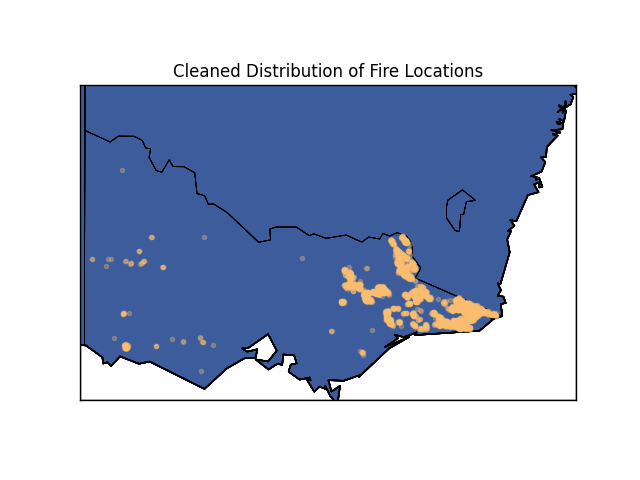
\includegraphics[width=\linewidth]{no_clustering.png}
  \caption{Cleaned Fired Distribution}
  % \label{fig:boat1}
\end{figure}

\subsubsection{Deploying SSA}

To deploy drones in a way that reaches the target of fast response, we
first need to quantify the target using one index, which we define it as
weighted covering lost(WCL).

\begin{equation}
WCL=\sum_j \Bigg(\int _{x0} ^{x1}  { (x-r_c)\cdot (1-p_{j,x})} \cdot vs_{j,x} \Bigg) \  dx \\ \\
\end{equation}

To simplify our model, we assume \(vs_{j,x}=v\), which is a stable
value, then we have.

\begin{equation}
WCL=\sum_j \Bigg(\int _{x0} ^{x1}  { (x-r_c)\cdot p_{j,x}} \cdot  v  \  dx\Bigg)^2
\end{equation}

In order to simply the model as well as simulate the distribution of
\(p_{j}\), we use Ridge Distribution to set \(p_{j,x}\), which is the
probability of rim of fire at the position which is \(x\) km from the
nearest SSA, as following

\begin{equation}
p_{j,x}=
\begin{cases}
\frac 1 2 - \frac 1 2 \sin \frac {\pi} {r_o}(x-\frac {r_o} {2} ) , & 0\le x \le r_0 \\ 
0 , & x > r_0
\end{cases}  
\end{equation}

This gives us

\begin{equation}
WCL=\sum_j \Bigg(\int _{x0} ^{x1}  { (x-r_c)\cdot (\frac 1 2 + \frac 1 2 \sin \frac {\pi} {r_o}(x-\frac {r_o} {2} ))} \cdot  v  \  dx \Bigg)^2
\end{equation}

We use the concept of substitution distance(\(sdist\)) to investigate
the deployment strategy.

\begin{equation}
sdist=\Bigg\| \int _{x0} ^{x1}  { (x-r_c)\cdot (\frac 1 2 + \frac 1 2 \sin \frac {\pi} {r_o}(x-\frac {r_o} {2} ))} \cdot  v  \  dx \Bigg\|
\end{equation}

We define \(sdist\) in a way that guarantees \(sdist\) is positively
correlated to \(x\) which is the distance to the center, that is, the
place where the nearest drone is deployed.

To balance economical costs and safety, we set a threshold for \(WCL\),
\(tWCL\) which is currently set to a certain value in our later
investigation, but it can be adjusted according to real situation. It
will be illustrated more thoroughly in the following section about
sensitivity and robustness. We use modified \(k-means\) cluster to
determine the positions of SSAs, which is described as follows
\begin{figure}[h!]
      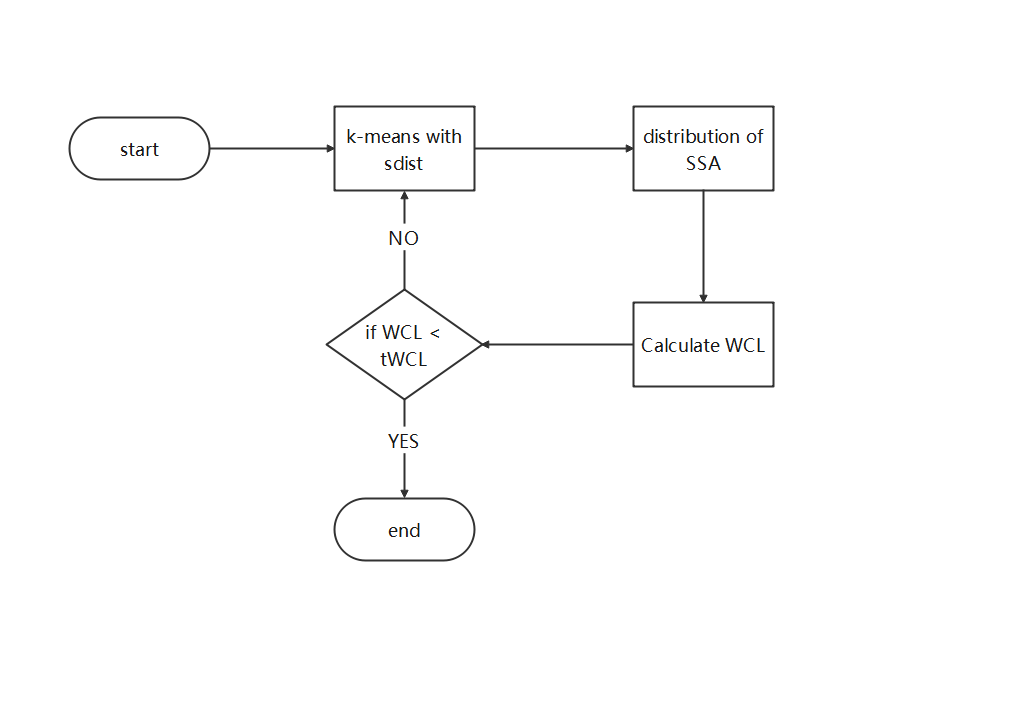
\includegraphics[width=\linewidth]{FlowChart2.png}
      \caption{deploy SSA flowchart}
      % \label{fig:boat1}
    \end{figure}
This allows us to cluster the locations to their respective drones.
k-means algorithm is used here since the \(sdist\) is positively
correlates to distance. So the correctness of the algorithm can be
ensured.
\begin{figure}[h!]
      \centering
      \begin{subfigure}[b]{0.4\linewidth}
        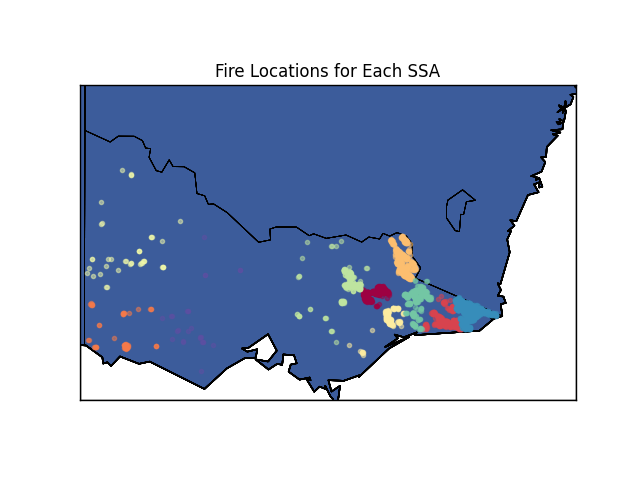
\includegraphics[width=\linewidth]{K-means_clustering.png}
        \caption{clustering of fire location}
      \end{subfigure}
      \begin{subfigure}[b]{0.4\linewidth}
        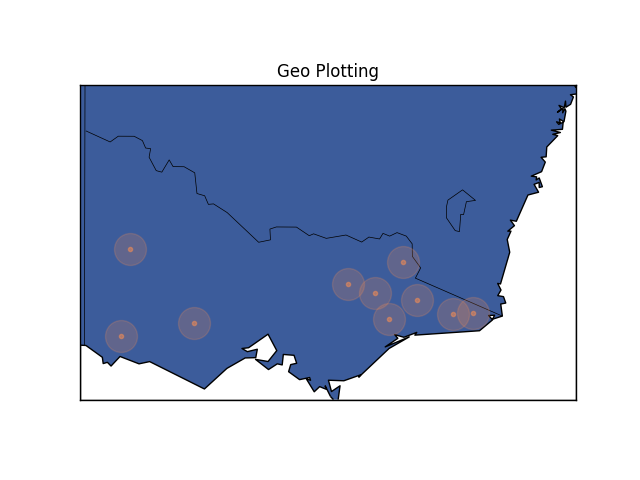
\includegraphics[width=\linewidth]{thermal_drones_deployment.png}
        \caption{SSA distribution}
      \end{subfigure}
      \caption{SSA and fire locations}
      \label{fig:coffee}
    \end{figure}
Given the fire location distribution, we plot the SSA's location as
above. The range is marked as well. It can be observed that the fire is
frequent and in large scale at the east of state of Victoria. Our
distribution perfectly fit the situation can reduce \(WCL\) to
acceptable level.

\subsubsection{Deploy Repeaters}

The second part of Fast Response Model is connecting all the SSAs using
the least repeaters. We solve this problem by divide and conquer and
with the help of minimum spanning tree.

For Dense Cluster, we choose to shrink several SSAs into one, since when
it's dense, one repeater can cover multiple SSAs. Then we build minimum
spanning tree on the repeaters.

For Sparse Cluster, we choose to build minimum spanning tree directly.

Combined both situation, we succeed in connecting all SSAs in a way that
guarantees both the stability of connection and minimum economic cost.

\paragraph{Dense Cluster}

For dense cluster, we choose shrink point strategy. For every dense
cluster which is formed by a set of SSAs, we use an algorithm to settle
the distribution of core repeater.

A core repeater is defined as, the repeater that can receive signal from
SSAs.

\begin{figure}[h!]
      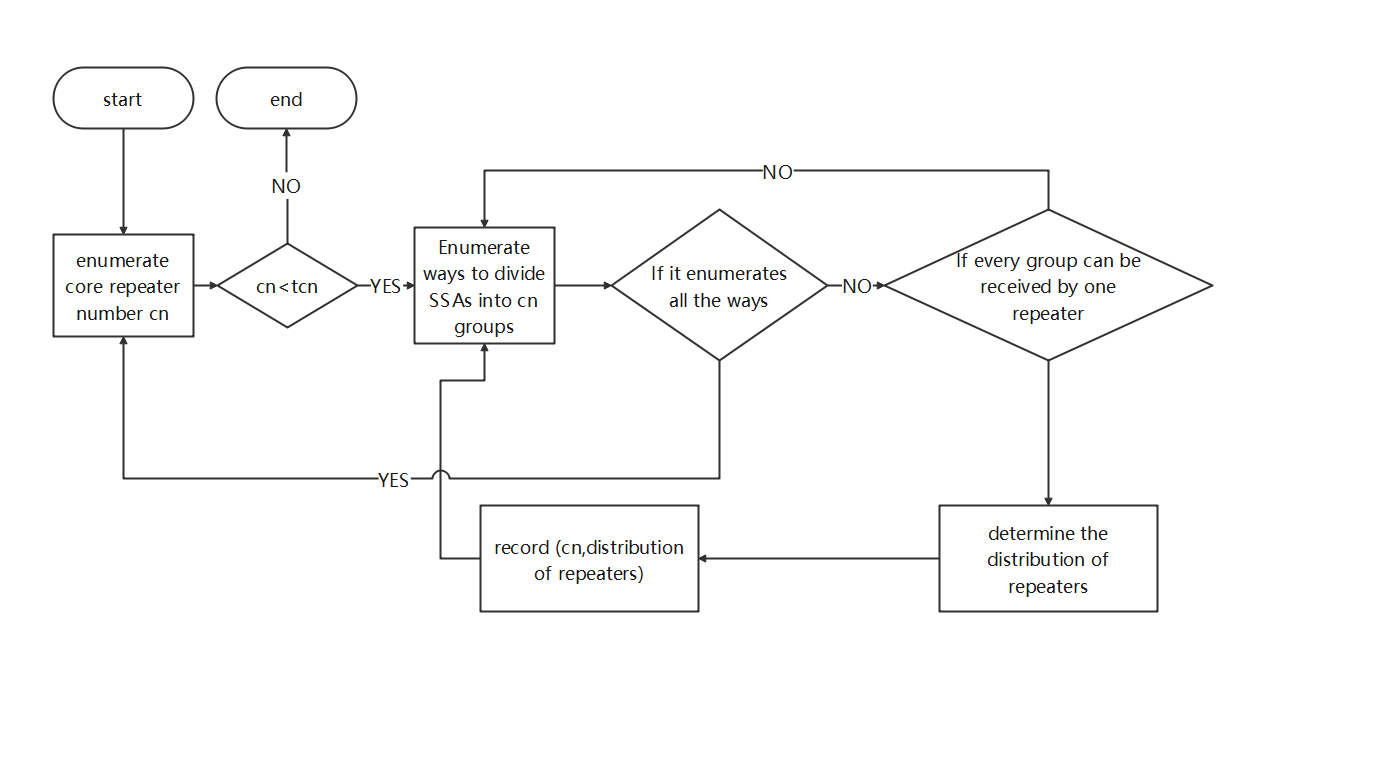
\includegraphics[width=\linewidth]{FlowChart3.png}
      \caption{Strategy for Dense Clutser}
      % \label{fig:boat1}
    \end{figure}

We want the combination of core repeaters to be in a way that allows the
minimum number of repeaters to be distributed and all the SSAs' signal
can be received. There seems to be no elegant solution to this problem
because it is \(NP\) problem. However, the small number of SSAs allows
us to use brute force to compute such distribution.

We define \(cn\) to be the number of core repeaters needed, \(nSSA\) to
be the SSA that are distributed, we define \(tcn\) to be the maximum
number of core repeaters that are allowed, it's obvious that
\(tcn \le nSSA\). For simplicity of implementation, we set \(tcn=nSSA\)

\paragraph{Sparse Cluster and Final Linking}

Now there are only sparse SSAs and sparse repeaters, it's natural to
link them by Kruskal algorithm to make a minimum spanning tree.

The first step is to build the graph with nodes and edges.

\begin{itemize}
\item
  Nodes are SSAs and repeaters, which is reasonable since they are
  sparse and can be discretized.
\item
  Edges have weight defined below. Considering if the range of drones
  are tangent to each other, the transmission stability will be lowered,
  we introduce transmission random factor \(trf\)
\end{itemize}

\begin{equation}
Ew_e= \max{ \Bigg(\Bigg\lceil \frac { dis_{i,j}  - 2r_c - trf_e} {2r_c} \Bigg\rceil,0\Bigg)}
\end{equation}

Transmission factor is defined below to reduce the situation where
ranges of drones are tangent, where \(randi(x)\) function is to randomly
produce a real number within interval \([0,x]\)

\begin{equation}
trf_e= randi \Bigg( 1- \Bigg(\Bigg\lceil \frac { dis_{i,j}  - 2r_c - trf_e} {2r_c} \Bigg\rceil -\frac { dis_{i,j}  - 2r_c - trf_e} {2r_c} \Bigg)\Bigg)
\end{equation}

Then we use Kruskal Algorithm\cite{kruskal} as described below to make a
spanning tree.

\newpage

\begin{figure}[h!]
      \centering
      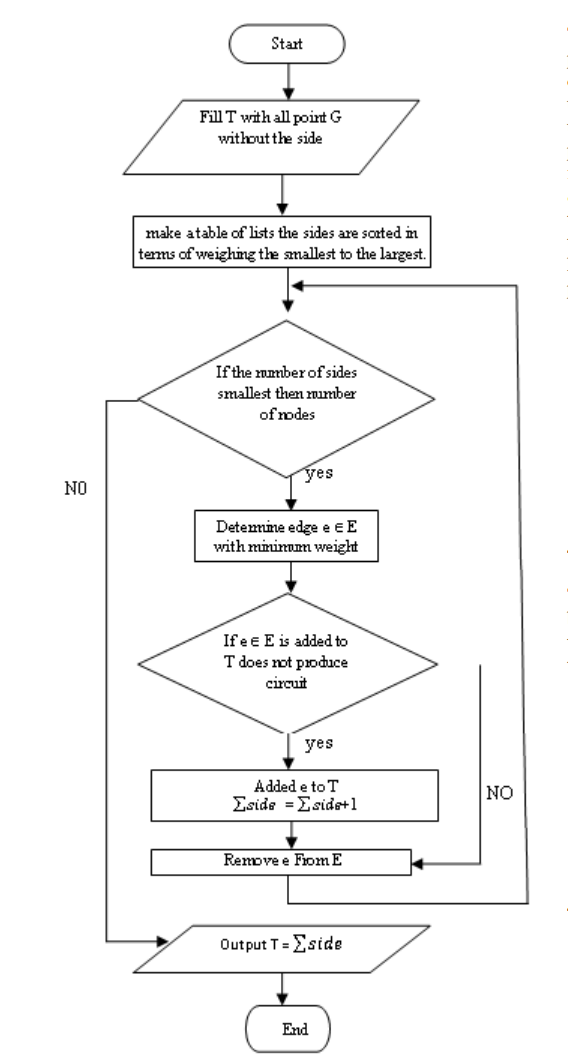
\includegraphics[width=.5\linewidth]{FlowChart4.png}
      \caption{Strategy for Dense Clutser}
      % \label{fig:boat1}
    \end{figure}



\begin{figure}[h!]
      \centering
      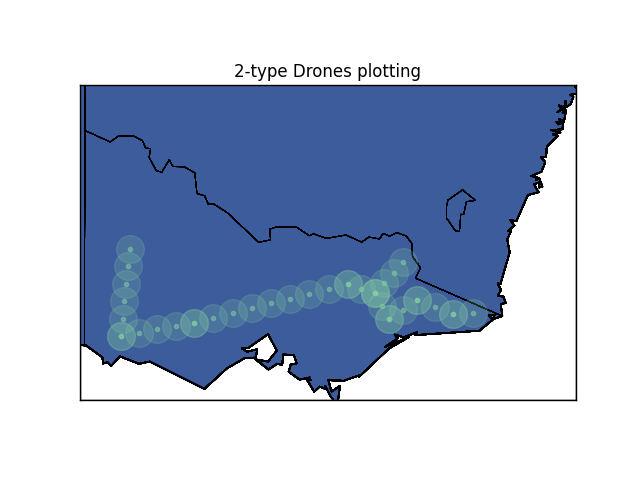
\includegraphics[width=.5\linewidth]{two_type.png}
      \caption{The general drone distribution}
      % \label{fig:boat1}
    \end{figure}

Because of the introduction of \(trf_e\) and the use of divide and
conquer strategy, the outcome is not only stable but also efficient as
shown.


\subsection{Fire Prediction Model}

\hypertarget{data-pre-processing}{%
\subsubsection{Data Pre-processing}\label{data-pre-processing}}

The data source used in this task is from Moderate-resolution Imaging
Spectroradiometer(MODIS) provided by NASA. The obtained time series data
of Australia wild-fire from 2003 to 2020 is saved in CSV format. The
task is to drop all data with confidence less than 80, and divide them
monthly. A high threshold for confidence is adopted to reduce the noise
of input data and make the prediction result more reliable. Given the
intensity of wildfires, it makes sense to combine data from the same
month to create heat maps. All mentioned operations are based on Pandas
in Python.\\
The data source used in this task is from Moderate-resolution Imaging
Spectroradiometer(MODIS) provided by NASA. The obtained time series data
of Australia wild-fire from 2003 to 2020 is saved in CSV format. The
task is to drop all data with confidence less than 80, and divide them
monthly. A high threshold for confidence is adopted to reduce the noise
of input data and make the prediction result more reliable. There are
two main reasons for selecting monthly divided data:

\begin{enumerate}
\def\labelenumi{\arabic{enumi}.}
\item
  Monthly divided data has a long time span, which can provide a long
  enough time series.
\item
  Monthly divided data has uniform time interval, which is convenient
  for statistical modeling of time series.
\end{enumerate}

All mentioned operations are based on Python's framework Pandas.

\hypertarget{build-map-with-fire-index}{%
\subsubsection{Build Map with Fire
Index}\label{build-map-with-fire-index}}

Australian Bureau of Statistics offers digital boundary files of all
states. By reading the shape file and monthly wild-fire data in MATLAB
R2021b, it's easy to use filterm function to drop all data points out of
the state Victoria, and map all points to a 109x185 matrix, where 20
terms in each dimension corresponding to one degree in geography.

The Heatmap function can build maps in an intuitive and easily
machine-learned form. By building maps for every month in 17 years, 204
maps are obtained. The figure below shows the wild fire in Victoria in
2003.

\begin{figure}[h!]
  \centering
\begin{subfigure}[b]{0.25\linewidth}
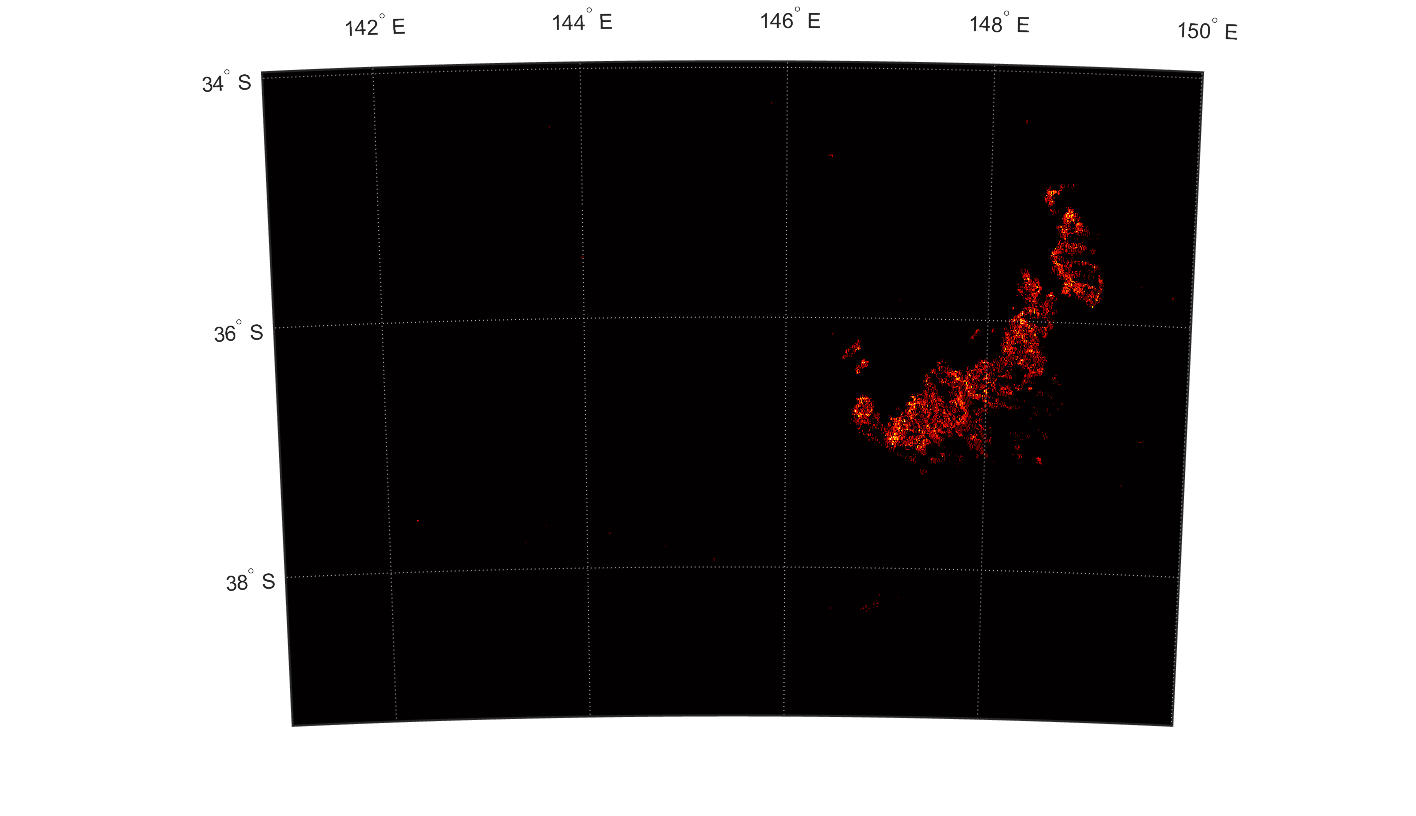
\includegraphics[width=\linewidth]{modis_2003_1_Australia.png}
\end{subfigure}
\begin{subfigure}[b]{0.25\linewidth}
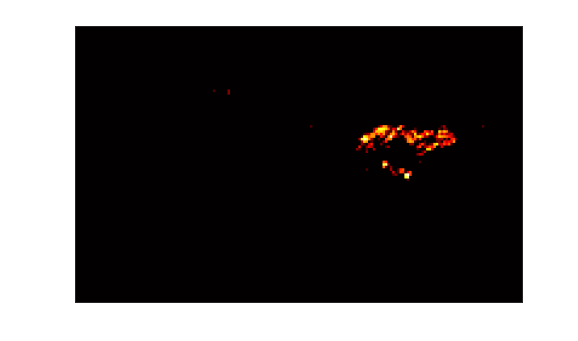
\includegraphics[width=\linewidth]{modis_2003_2_Australia.png}
\end{subfigure}
\begin{subfigure}[b]{0.25\linewidth}
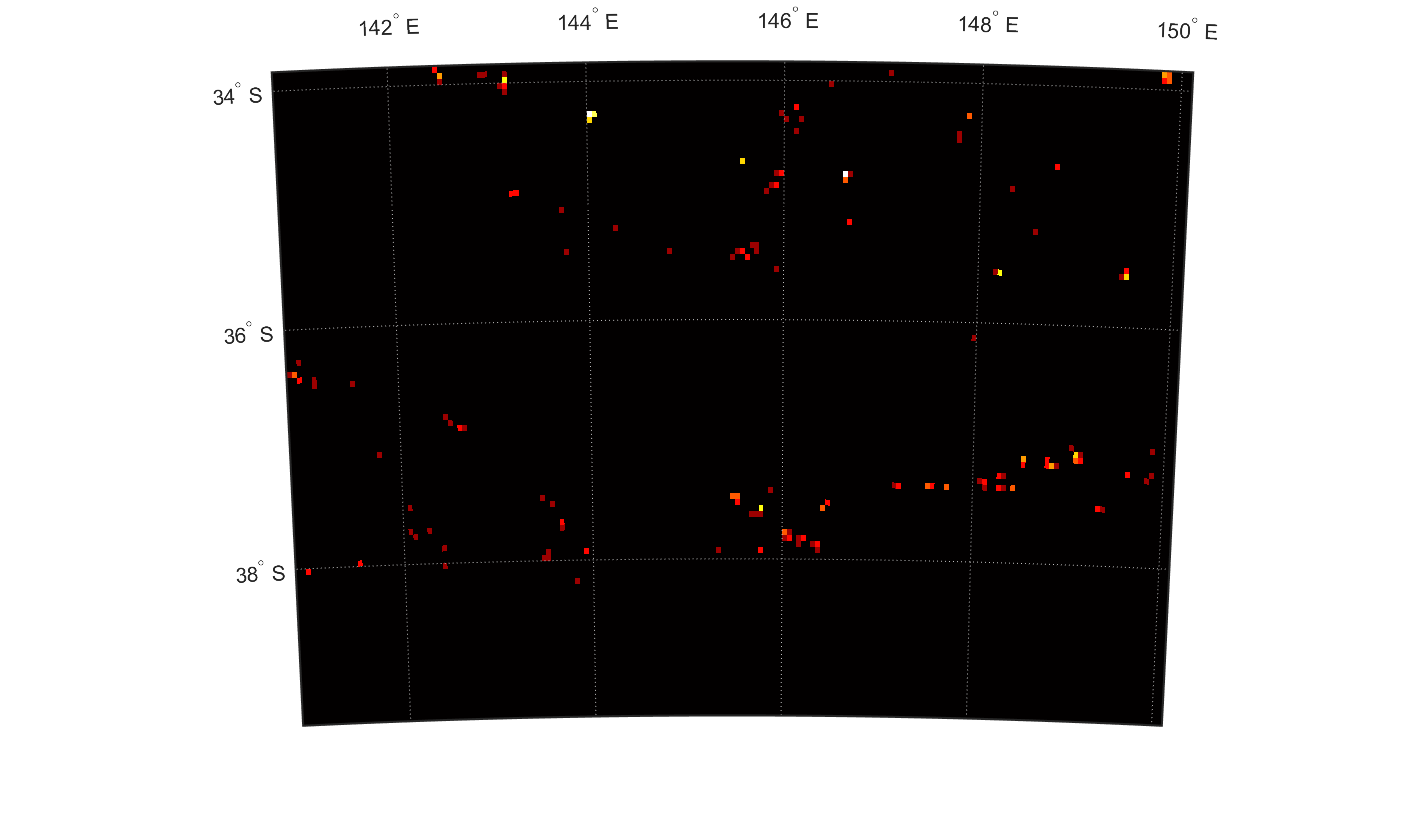
\includegraphics[width=\linewidth]{modis_2003_3_Australia.png}
\end{subfigure}
\begin{subfigure}[b]{0.25\linewidth}
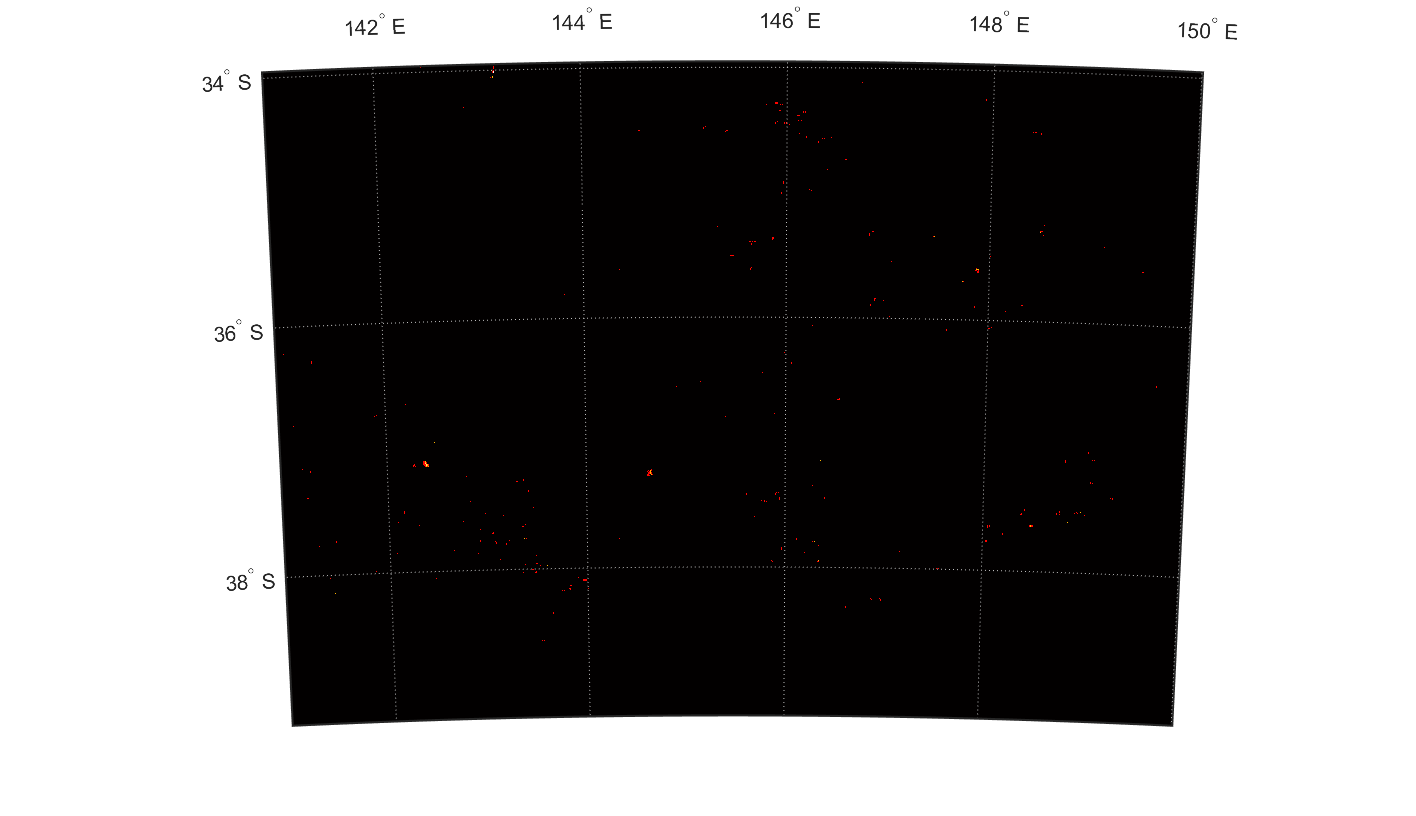
\includegraphics[width=\linewidth]{modis_2003_4_Australia.png}
\end{subfigure}
\begin{subfigure}[b]{0.25\linewidth}
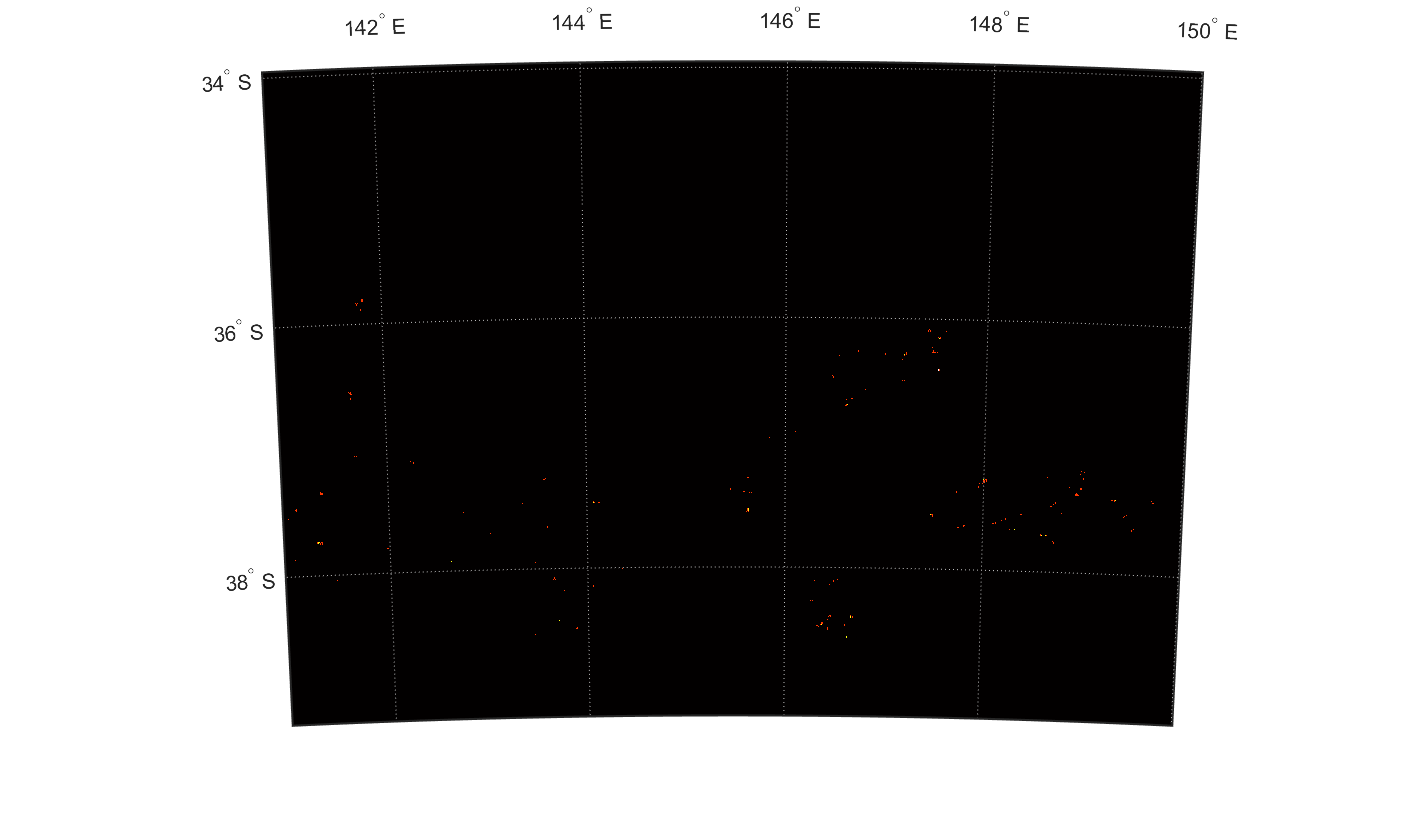
\includegraphics[width=\linewidth]{modis_2003_5_Australia.png}
\end{subfigure}
\begin{subfigure}[b]{0.25\linewidth}
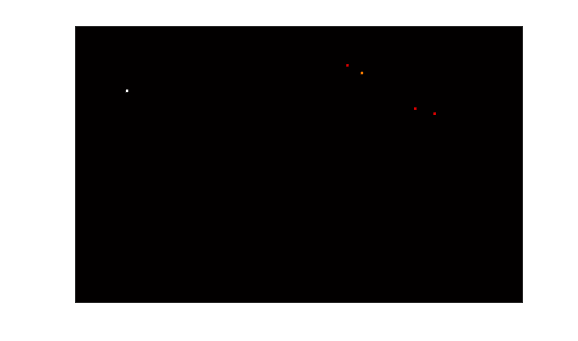
\includegraphics[width=\linewidth]{modis_2003_6_Australia.png}
\end{subfigure}
\begin{subfigure}[b]{0.25\linewidth}
  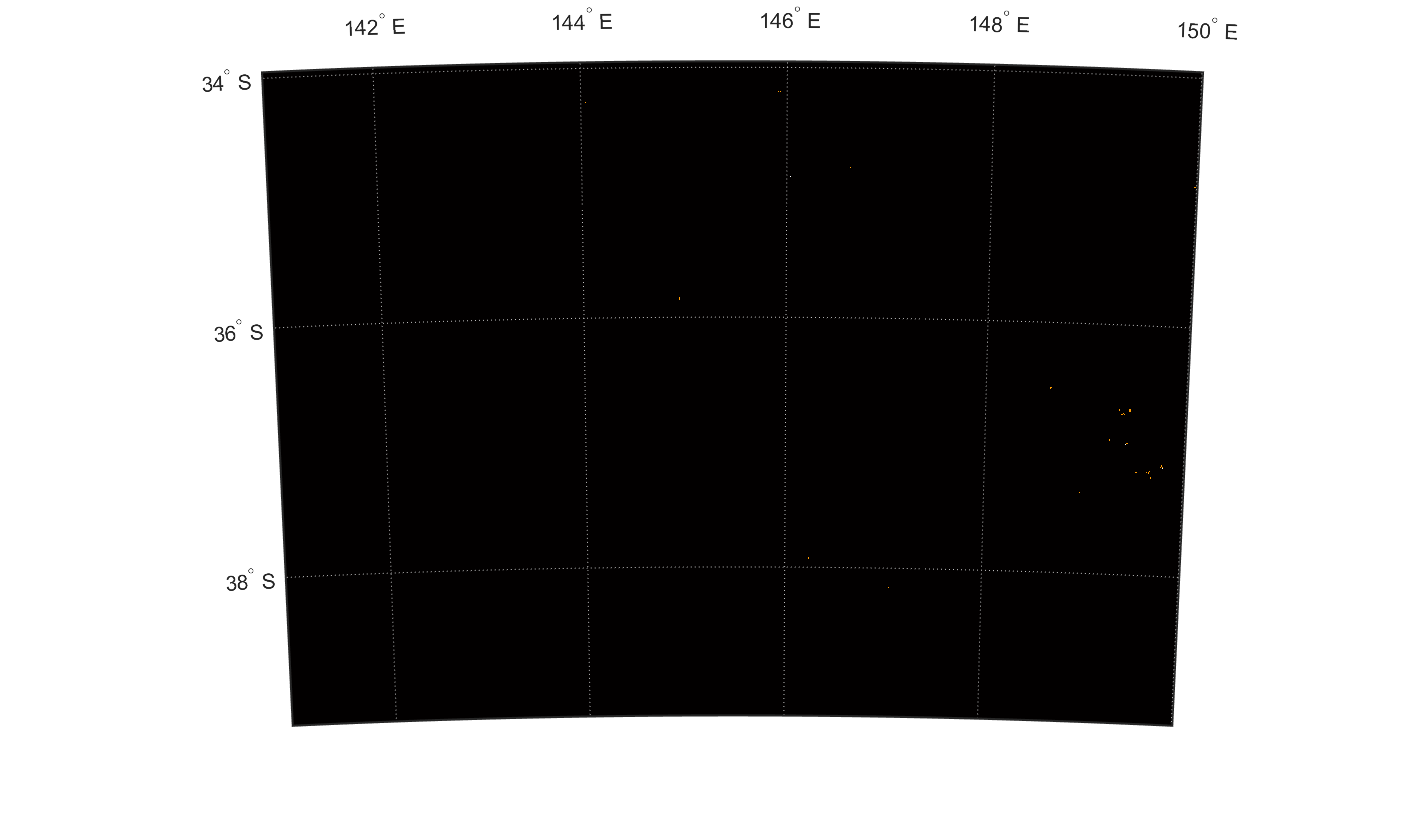
\includegraphics[width=\linewidth]{modis_2003_7_Australia.png}
  \end{subfigure}
  \begin{subfigure}[b]{0.25\linewidth}
  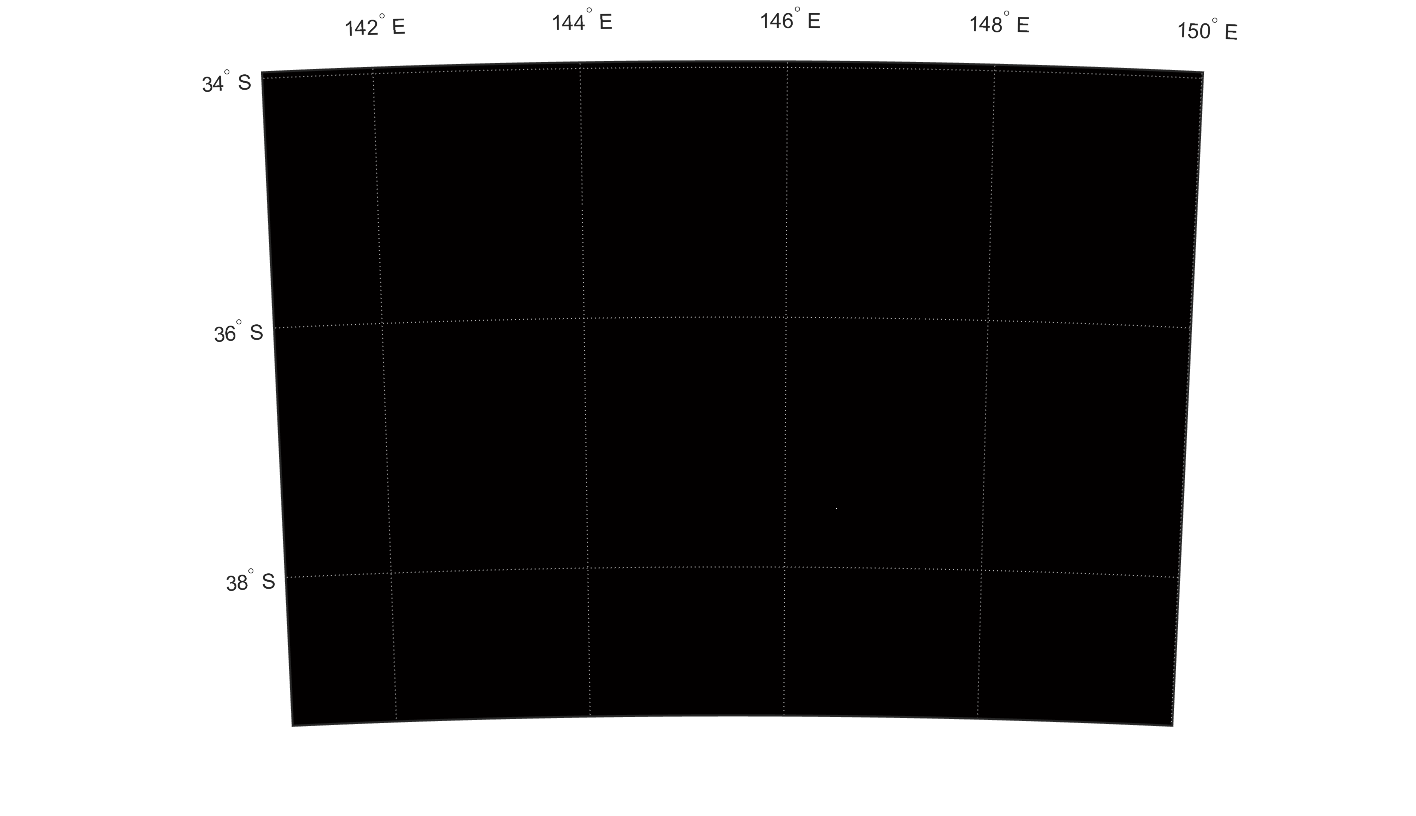
\includegraphics[width=\linewidth]{modis_2003_8_Australia.png}
  \end{subfigure}
  \begin{subfigure}[b]{0.25\linewidth}
  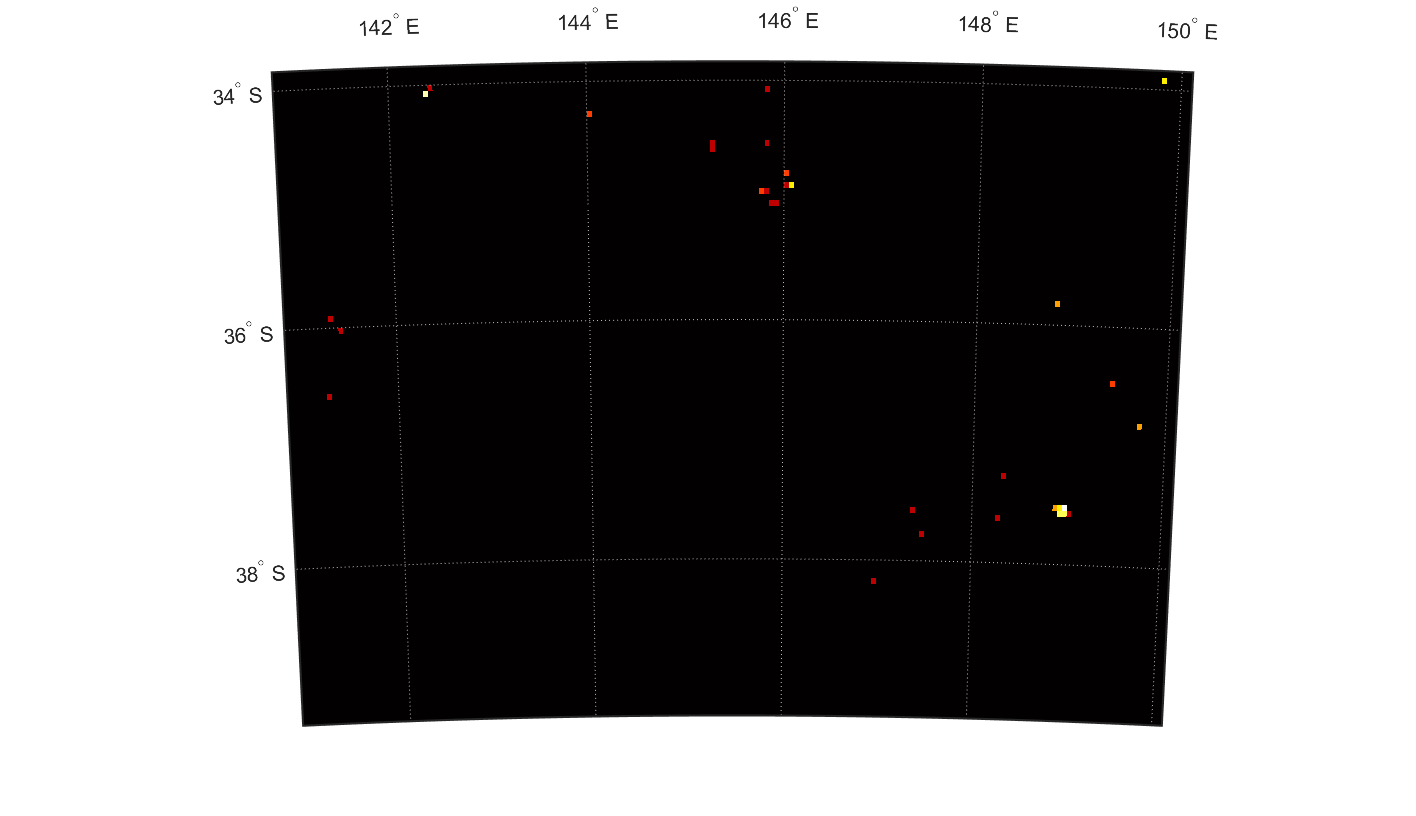
\includegraphics[width=\linewidth]{modis_2003_9_Australia.png}
  \end{subfigure}
  \begin{subfigure}[b]{0.25\linewidth}
  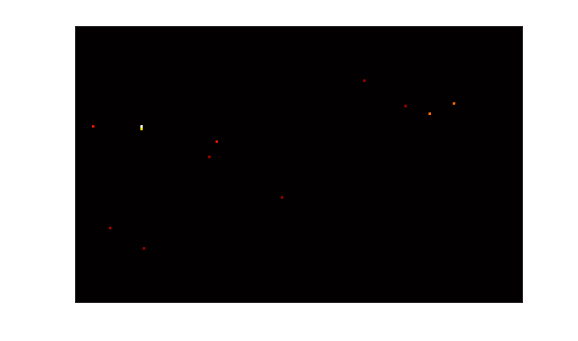
\includegraphics[width=\linewidth]{modis_2003_10_Australia.png}
  \end{subfigure}
  \begin{subfigure}[b]{0.25\linewidth}
  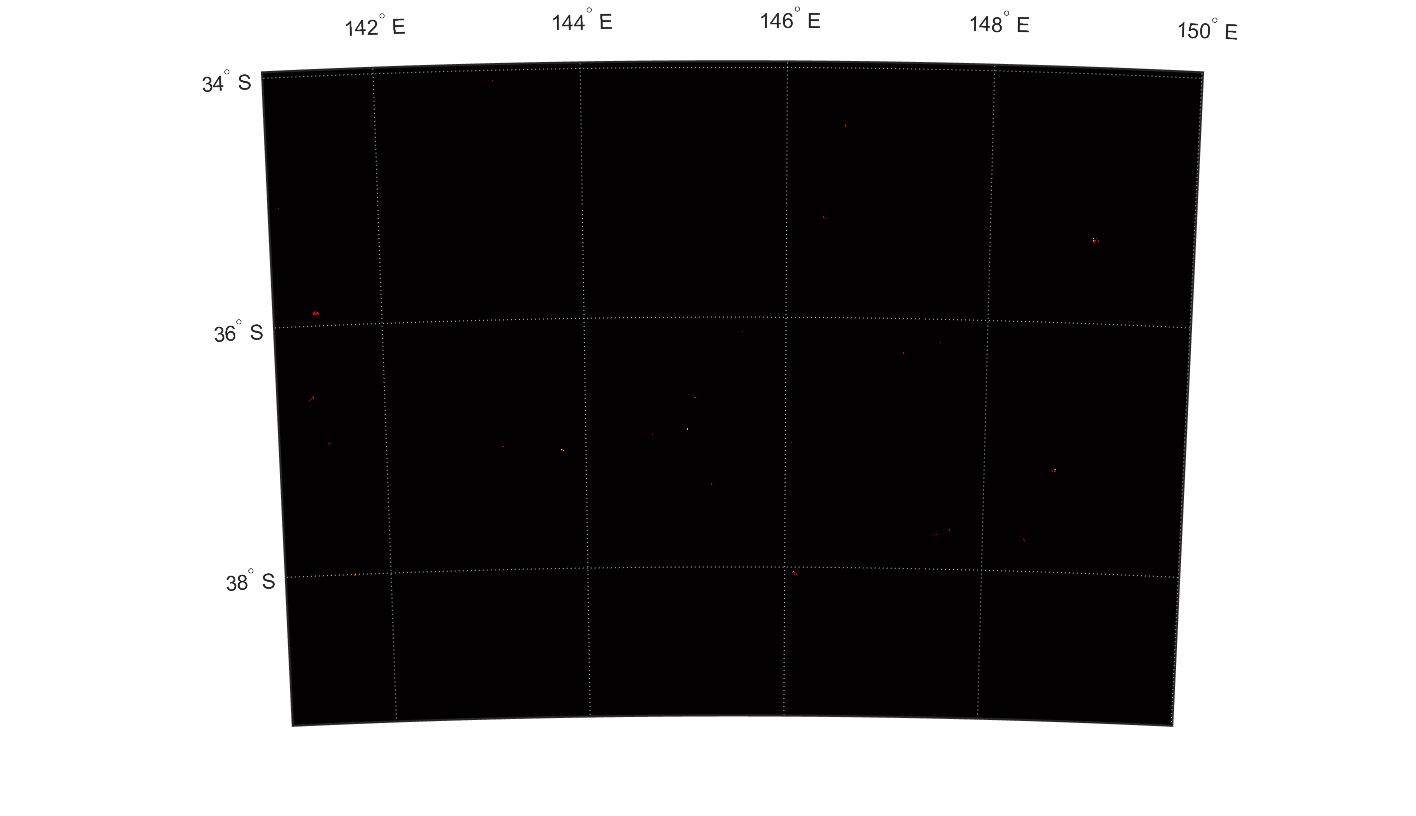
\includegraphics[width=\linewidth]{modis_2003_11_Australia.png}
  \end{subfigure}
  \begin{subfigure}[b]{0.25\linewidth}
  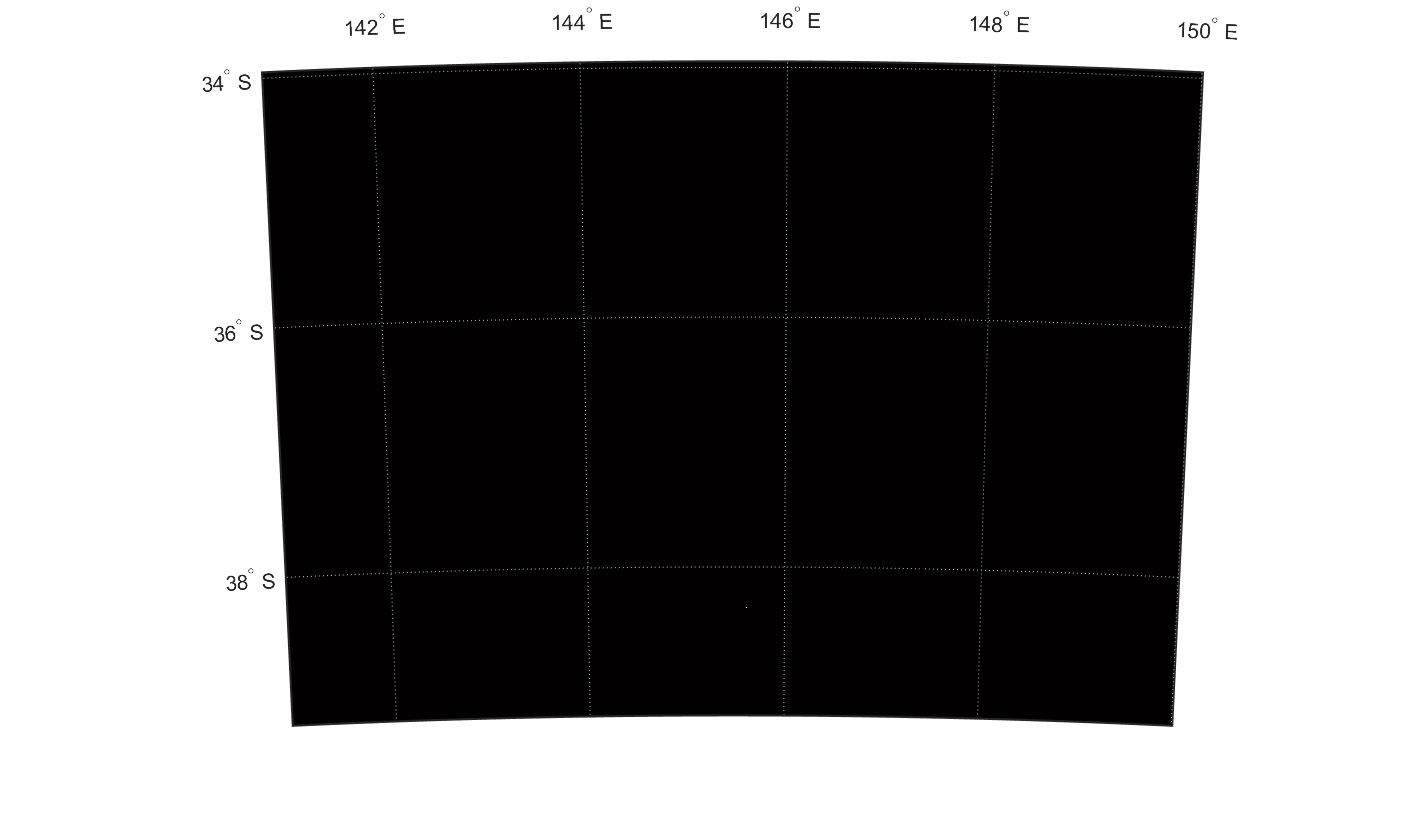
\includegraphics[width=\linewidth]{modis_2003_12_Australia.png}
  \end{subfigure}
\caption{Wild Fire in Victoria in Year 2003}
  \label{fig:1-12}
\end{figure}
The RGB channel values in the picture are given by the following
formula:
\begin{equation}
R_{x,y}=\left\{
\begin{array}{lr}
\left \lfloor 255\frac{3\root4\of{{heat}_{x,y}}}{\max(\root4\of {heat})} \right \rfloor & \root4\of{{heat}_{x,y}}<\frac{1}{3}\max(\root4\of {heat})  \\  
255 & \root4\of{{heat}_{x,y}}\ge\frac{1}{3}\max(\root4\of {heat})
\end{array}  
\right.
\end{equation}
\begin{equation}
G_{x,y}=\left\{
\begin{array}{lr}
0&\root4\of{{heat}_{x,y}}\le\frac{1}{3}\max(\root4\of {heat})\\
\left \lfloor 255\big(\frac{3\root4\of{{heat}_{x,y}}}{\max(\root4\of {heat})}-1\big) \right \rfloor&\frac{1}{3}\max(\root4\of {heat})<\root4\of{{heat}_{x,y}}<\frac{2}{3}\max(\root4\of {heat})  \\  
255&\root4\of{{heat}_{x,y}}\ge\frac{2}{3}\max(\root4\of {heat})
\end{array}  
\right.
\end{equation}
\begin{equation}
B_{x,y}=\left\{
\begin{array}{lr}
0&\root4\of{{heat}_{x,y}}<\frac{2}{3}\max(\root4\of {heat})\\
\left \lfloor 255\big(\frac{3\root4\of{{heat}_{x,y}}}{\max(\root4\of {heat})}-2\big) \right \rfloor&\root4\of{{heat}_{x,y}}\ge\frac{2}{3}\max(\root4\of {heat})  
\end{array}  
\right.
\end{equation}
\hypertarget{time-series-construction}{%
\subsubsection{Time series
construction}\label{time-series-construction}}

After removing the white edges around the image, 204 images are read into Python and constructed into a five-dimensional tensor
with size (192,12,3,185,109). 204-12=192 time steps are saved in the tensor, and each time step contains 12 batches with 3 channels, 
185 of pixel in width and 109 in height.In this paper, the sliding window method\cite{7785326} was used to divide the MODIS 
data used in the study into the input and output sets of supervised training. In terms of time, the input sequence length is 12 images 
of one-year sequential data, the output sequence length is 1 image of sequential data in the next month, and the sliding step length is 
one image in one month. For example, the data of 2003 is the input, the data of January 2004 is the output, the input of the next sliding 
window is the data of February 2003 to January 2004, the output is the data of February 2004, and so on to the last year of the sequence.

\hypertarget{convlstm}{%
\subsubsection{ConvLSTM}\label{convlstm}}

Time series data prediction refers to learning past time series and
predicting future changes. Traditional Neural networks cannot solve the
problem of time-axis variation, so RNN (Recurrent Neural network) is
developed \cite{JORDAN1997471}.

However, due to the poor performance of classical RNN in extracting long
time series information and the limited time series information
extracted, Hochreiter developed LSTM network model \cite{10.1162/neco.1997.9.8.1735}. In classical RNN, gates structure is added to selectively add
and delete the past timing information, and input gate, output gate and
forgetting gate are added to control the input and output of data of
this unit (an LSTM cell is a basic unit) and the increase and decrease
of the output information of the previous unit respectively. The LSTM
formula is expressed as follows:
\begin{equation}
\mathbf{i}_t=\sigma(\mathbf{W}_{xi}\mathbf{X}_{t}+\mathbf{W}_{hi}\mathbf{H}_{t-1}+\mathbf{W}_{ci}\circ\mathbf{C}_{t-1}+b_i)
\end{equation}
\begin{equation}
\mathbf{f}_t=\sigma(\mathbf{W}_{xf}\mathbf{X}_{t}+\mathbf{W}_{hf}\mathbf{H}_{t-1}+\mathbf{W}_{cf}\circ\mathbf{C}_{t-1}+b_f) 
\end{equation}
\begin{equation}
\mathbf{C}_t=\mathbf{f}_{t}\circ\mathbf{C}_{t-1}+\mathbf{i}_t\circ\tanh(\mathbf{W}_{xc}\mathbf{X}_{t}+\mathbf{W}_{hc}\mathbf{H}_{t-1}+b_c)
\end{equation}
\begin{equation}
\mathbf{o}_t=\sigma(\mathbf{W}_{xo}\mathbf{X}_{t}+\mathbf{W}_{ho}\mathbf{H}_{t-1}+\mathbf{W}_{co}\circ\mathbf{C}_{t-1}+b_o)
\end{equation}
ConvLSTM is a variant of LSTM proposed on the basis of LSTM. It replaces
the fully connected state between the input layer and the hidden layer
and between the hidden layer and the hidden layer of LSTM with the
convolution connection, which makes full use of the spatial information
that LSTM cannot. LSTM needs to transform image data into
one-dimensional vector when processing image data, and cannot process
spatial structure information of original image data. Compared with LSTM
model,Conv LSTM can better extract spatial and temporal structure
information from time series images. ConvLSTM model formula is expressed
as follows:
\begin{equation}
\mathbf{i}_t=\sigma(\mathbf{W}_{xi}*\mathbf{X}_{t}+\mathbf{W}_{hi}*\mathbf{H}_{t-1}+\mathbf{W}_{ci}\circ\mathbf{C}_{t-1}+b_i)
\end{equation}
\begin{equation}
\mathbf{f}_t=\sigma(\mathbf{W}_{xf}*\mathbf{X}_{t}+\mathbf{W}_{hf}*\mathbf{H}_{t-1}+\mathbf{W}_{cf}\circ\mathbf{C}_{t-1}+b_f) 
\end{equation}
\begin{equation}
\mathbf{C}_t=\mathbf{f}_{t}\circ\mathbf{C}_{t-1}+\mathbf{i}_t\circ\tanh(\mathbf{W}_{xc}*\mathbf{X}_{t}+\mathbf{W}_{hc}*\mathbf{H}_{t-1}+b_c)
\end{equation}
\begin{equation}
\mathbf{o}_t=\sigma(\mathbf{W}_{xo}*\mathbf{X}_{t}+\mathbf{W}_{ho}*\mathbf{H}_{t-1}+\mathbf{W}_{co}\circ\mathbf{C}_{t-1}+b_o)
\end{equation}
The symbol meaning in the formula is the same as that in LSTM. The full
connection of input variables is replaced by convolution operation.
According to the internal structure of ConvLSTM in figure, it can be
seen that input gate, output gate and forgetting gate all carry out
convolution operation for input and hidden layer.
\begin{figure}[h!]
\centering
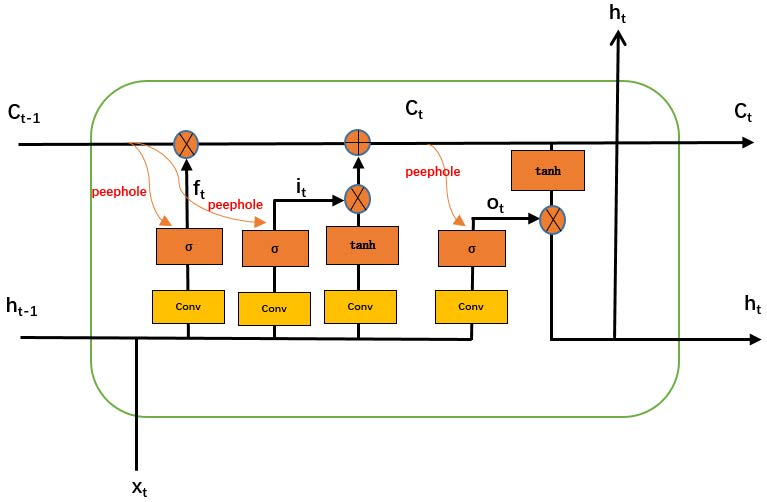
\includegraphics[width=0.7\linewidth]{Structure_of_ConvLSTM_Cell.jpg}
\caption{Structure of ConvLSTM Cell}
\end{figure}

\(\mathbf{W}_{ci}\circ\mathbf{C}_{t-1}\),
\(\mathbf{W}_{cf}\circ\mathbf{C}_{t-1}\) and
\(\mathbf{W}_{co}\circ\mathbf{C}_{t-1}\) in the formula indicate
that the input, output and forgetting gates are connected to the
Peephole\cite{861302} of the previous cellular state. As shown in
the figure, the Peephole connection adds cell state information to each
gate. Since the unit may have a door state of 0, which results in a lack
of important information, adding the Peephole operation can cover this
shortcoming.

Based on the deep learning framework Pytorch, the ConvLSTM is
constructed using Python language, and the experimental equipment
environment is NVIDIA GeForce GTX1080 GPU.
\begin{figure}[h!]
  \centering
  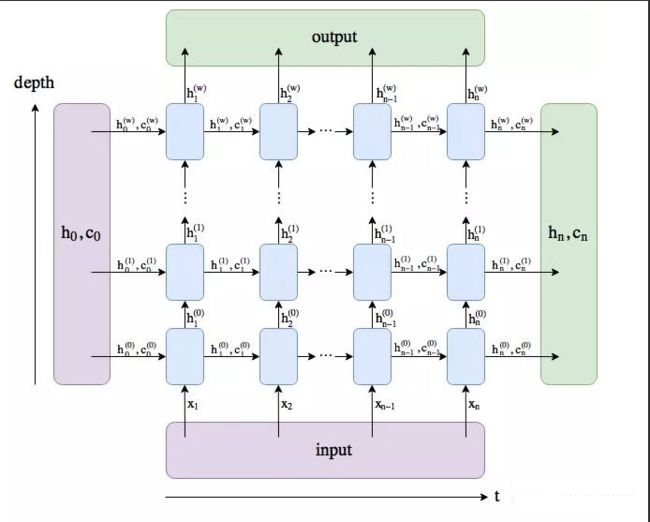
\includegraphics[width=0.7\linewidth]{Structure_of_ConvLSTM_Network.jpg}
  \caption{Structure of ConvLSTM Network}
  \end{figure}

  For the same prediction accuracy, the larger the convolution kernel is, 
  the higher the spatial resolution of the required image data is. 
  MODIS data are of low resolution, so the convolution kernel used in this paper is 3×3. In the experiment,
   the Batch Size was set to 12, the optimizer was Adam, the loss function was the mean square loss function, 
   the learning rate was set to 0.001, and the training epoch was 200.
\hypertarget{model-fitting}{%
\subsubsection{Model Fitting}\label{model-fitting}}



\subsection{Pearl and Spur Model}
\subsubsection{Pearl Model}

2019, Victoria, Australia suffered a severe bushfire. On 1th January,
houses were burned to the groung as NSW fire spread to Corryong in the
northern Victoria. Corryong, the town which is surrounded by Mount Mitta
and Wabba Wilderness Park was in great in danger.

In order to determine our model for optimizing the locations of hovering
VHF/UHF radio-repeater drones for fires of different sizes on different
terrains, we need to consider various terrains, including hills, plain
and mountains. Corryong, the city lying in the basin, is perfect for our
optimization. Therefore, we will take Corryong for an ecxample to
explain our location strategy.

We assume the fire is happening in the area surrounded by the red
circle, the area is much larger than the drones hovering range. Our
basic strategy is to supervise the edge of the bushfire area. Therefore
, we will need the "Boots-on-the-ground'' Forward Teams be at the front
lines of the fire events carrying the VHF/UHF. Conisdering various
situations, there is always no definitely perfect strategy to guide the
teams to distribute. Thus, we consider all random situations for the
distribution of the firefighters.

\begin{figure}[h!]
      \centering
      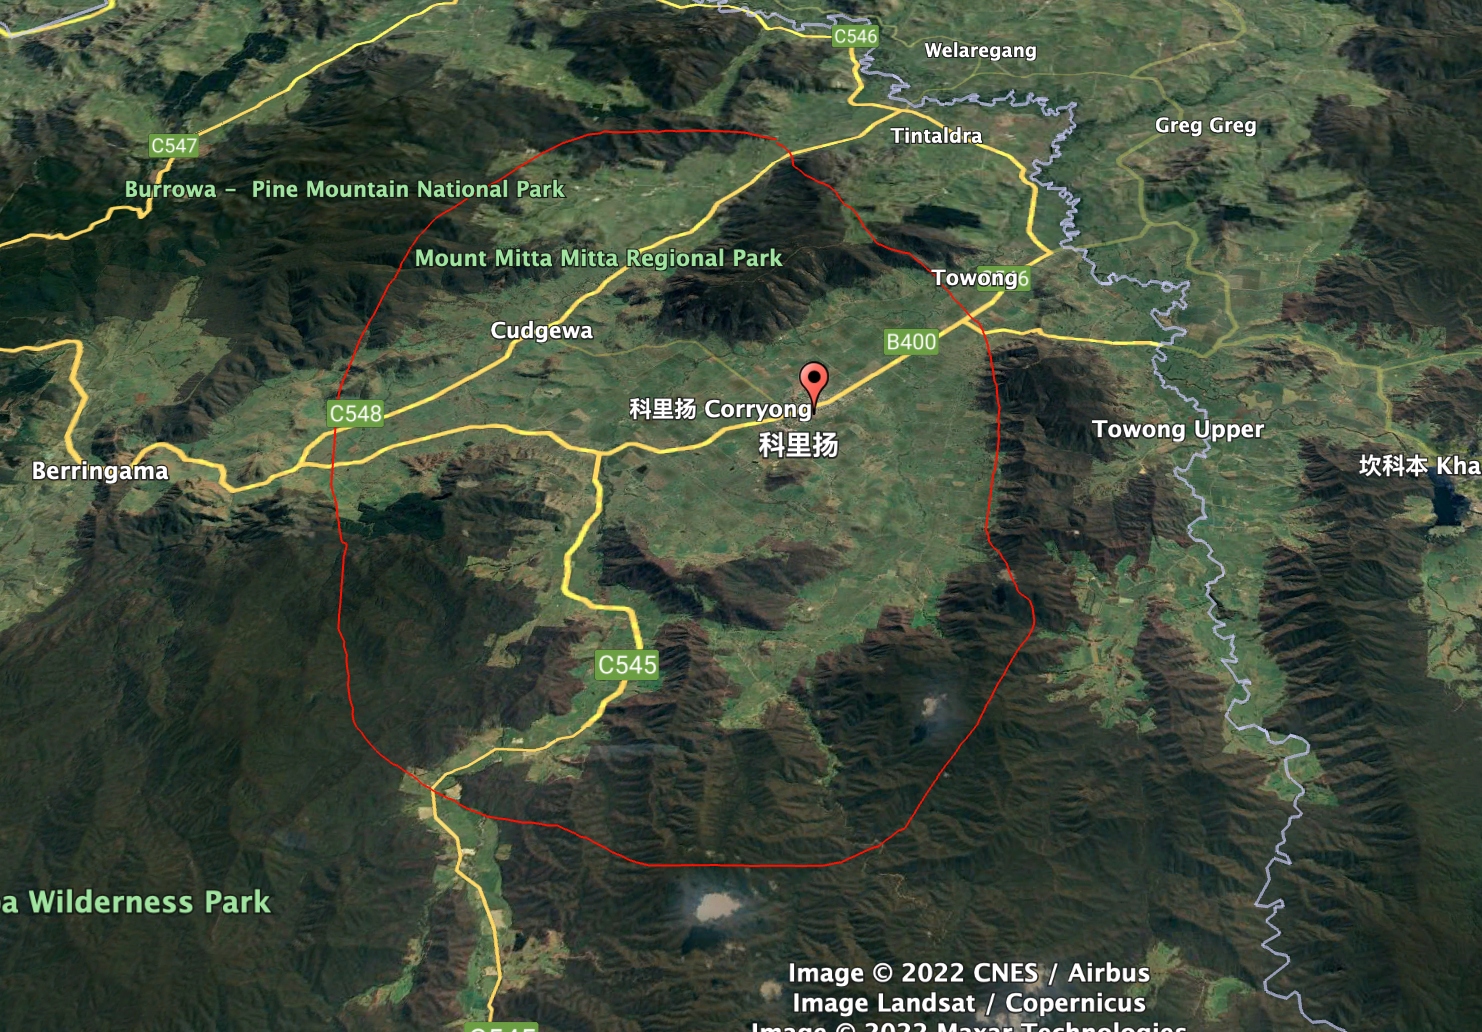
\includegraphics[width=.5\linewidth]{terrain.png}
      \caption{Hypothetical bush fire area happening in the Corryong}
    \end{figure}

Based on the bushfire area, we can get a latitude function along the
periphery of the enclosed area, which is shown as below.
\begin{figure}[h!]
      \centering
      \captionsetup{justification=centering}
      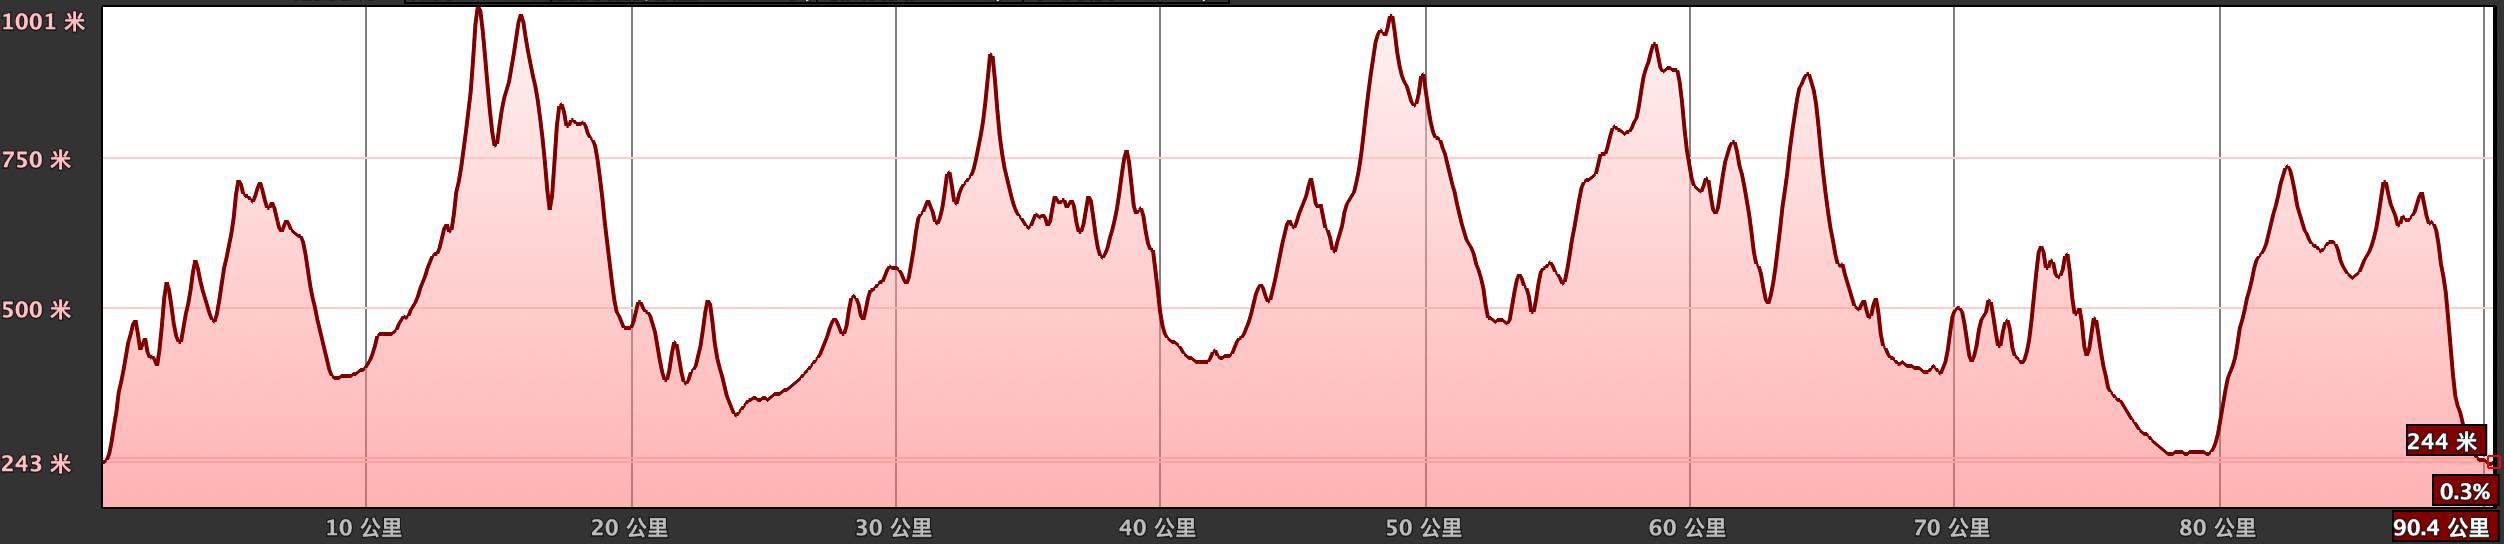
\includegraphics[width=\linewidth]{latitude.png}
      \caption{latitude along the peripher}
      \end{figure}
    
This function has a x-axis which represents the distance along the
periphery of the area from certain point, and a y-axis which represents
the latitudes of the point. Considering the effect of latitude is
significant to the height of drones should be, so that they avoid the
signal loss caused by terrains as possible as they can.

We choose to use the Monte-Carlo algorithm to analyze the effect of
firefighters' distribution to the locations of the hovering drones. For
the first step, we will distribute some fire fighter at the front line
of the bushfire area for simulation. Below is one condition considered.

\begin{figure}[h!]
      \centering
      \captionsetup{justification=centering}
      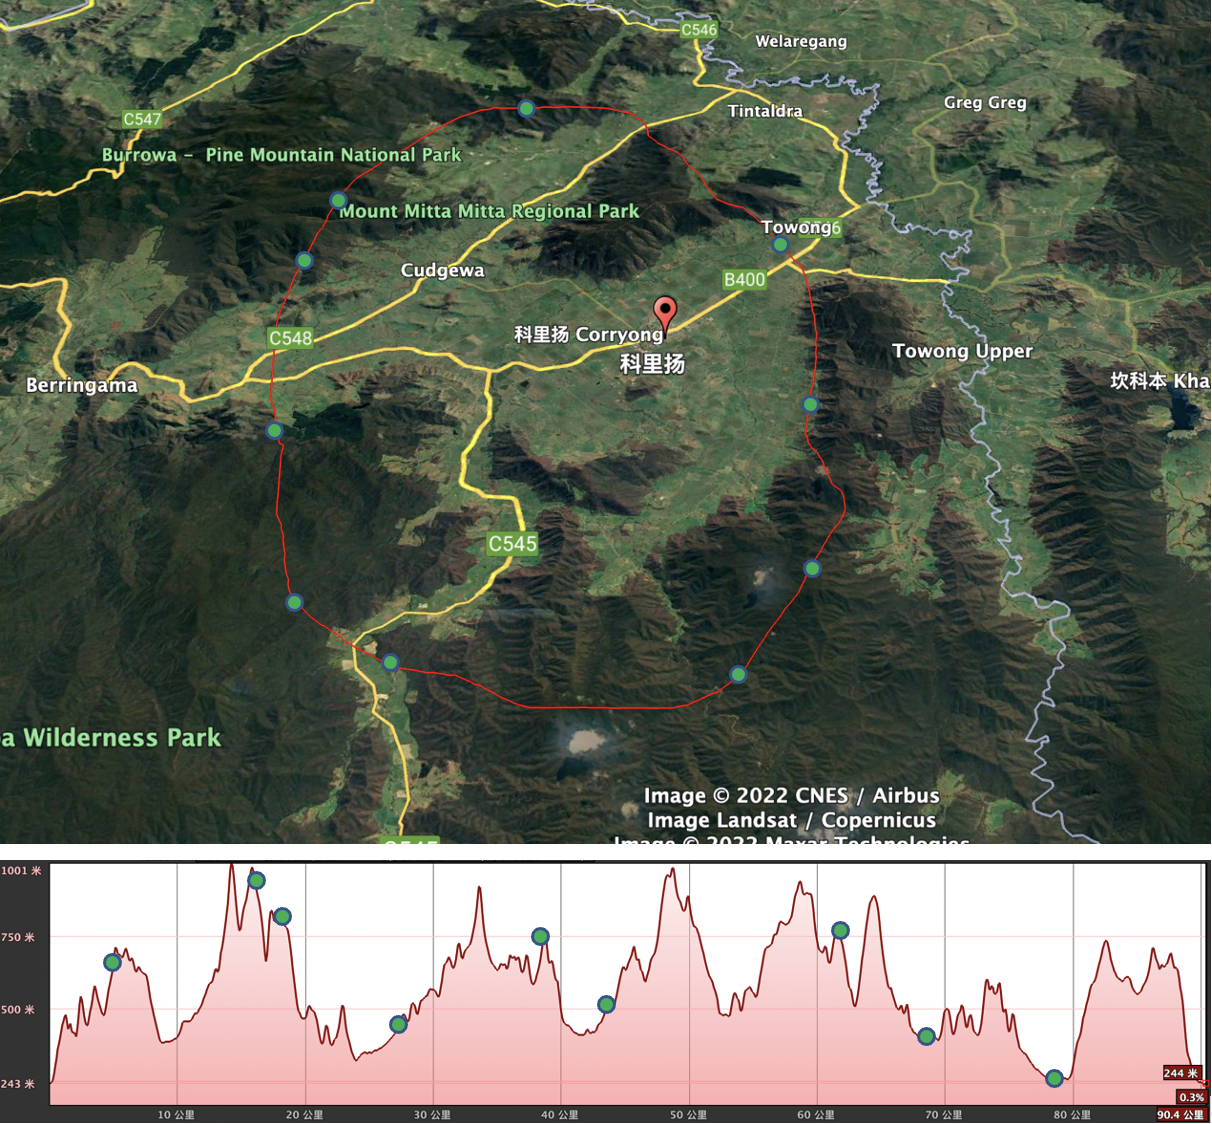
\includegraphics[width=.7\linewidth]{human_simulation.png}
      \caption{Distribute fire fighters ramdomly}
      \end{figure}
      
Green points represent fire fighters carrying VHF/UHF (9 firefighters in simulation)

From the results provided by the Google earth pro, we obtain the
function of the distance along the periphery and the latitude

\begin{equation}
H(x_i)
\end{equation}

\subsubsection{Drones' locations strategy explanation}

There are some basic principles we need to follow to settle the drones

\begin{enumerate}
\def\labelenumi{\arabic{enumi}.}
\item
  The distance of two drones can't be over 20 km, which is maximum range
  that transceivers can spread and receive.
\item
  Every individual fire fighter must be received by at least one drone
  so that they can keep connected.
\item
  Drones should be settled along the periphery of the bushfire area.
\item
  Drones should be in the reasonable height so that the radio signal
  won't be interrupted by the terrain obstacles, for example hills
  between.
\end{enumerate}

Therefore we have the drones' settling strattegy as below

\begin{figure}[h!]
      \centering
      \captionsetup{justification=centering}
      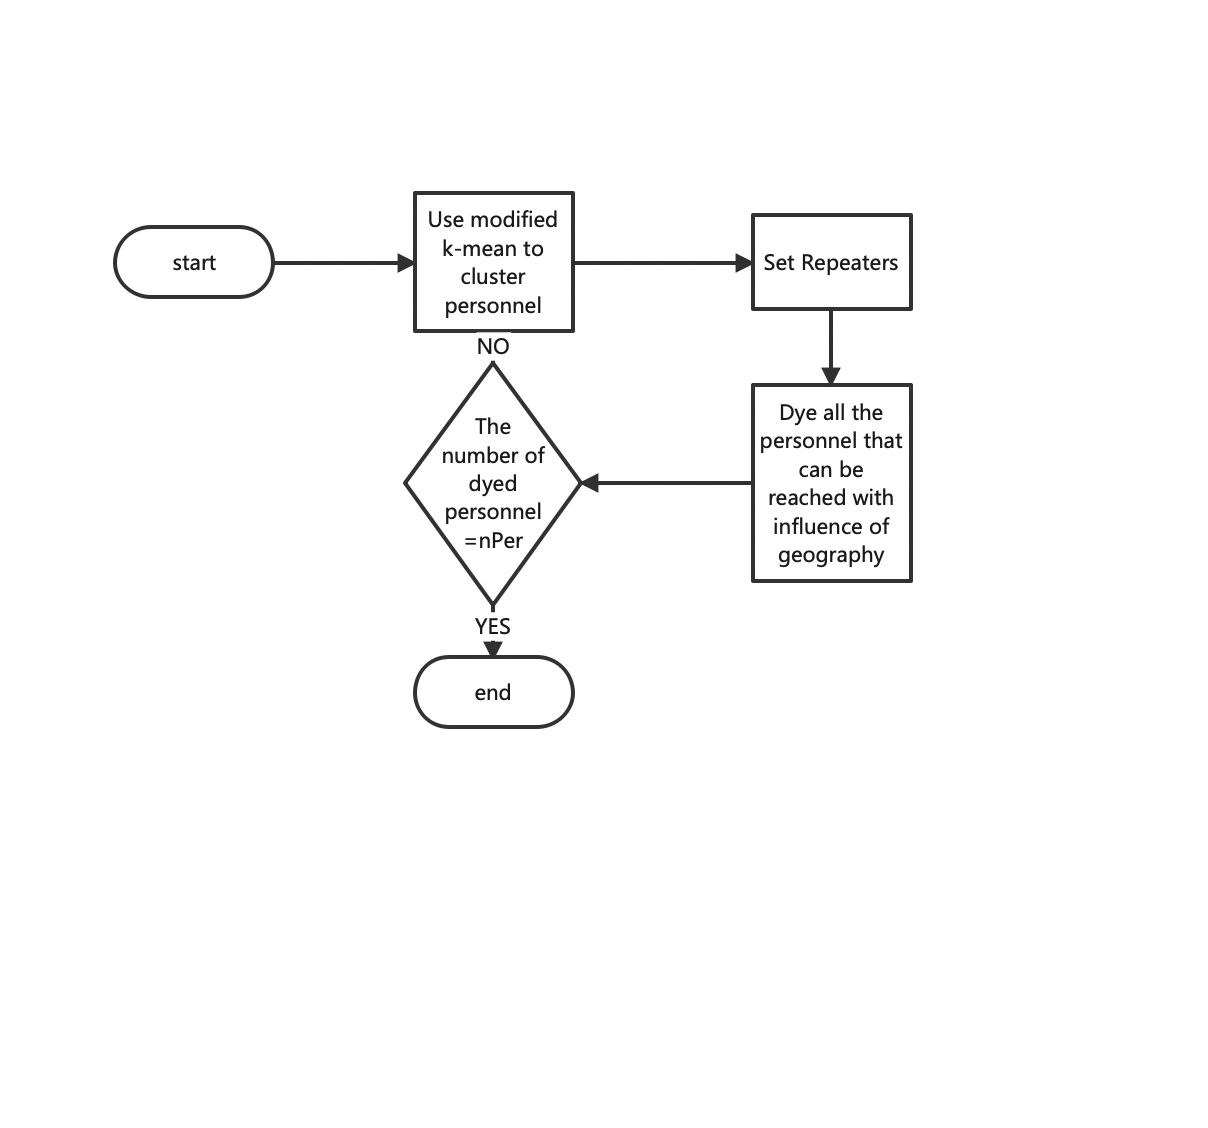
\includegraphics[width=.5\linewidth]{mindmap.png}
      \caption{mindmap of drones strategy}
      \end{figure}
    
\begin{equation}
sdist=
\end{equation}

\(x_i\) means the location along the periphery; \(d_i\) represents the
distance required along the periphery that makes the point \(x_{i-1}\)
moving forward for 20km in the actual distance; sigma is the factor
which make drones get closer to the previous one due to the terrain.

After these analysis, we can get the distribution of the drones:

\begin{figure}[h!]
      \centering
      \captionsetup{justification=centering}
      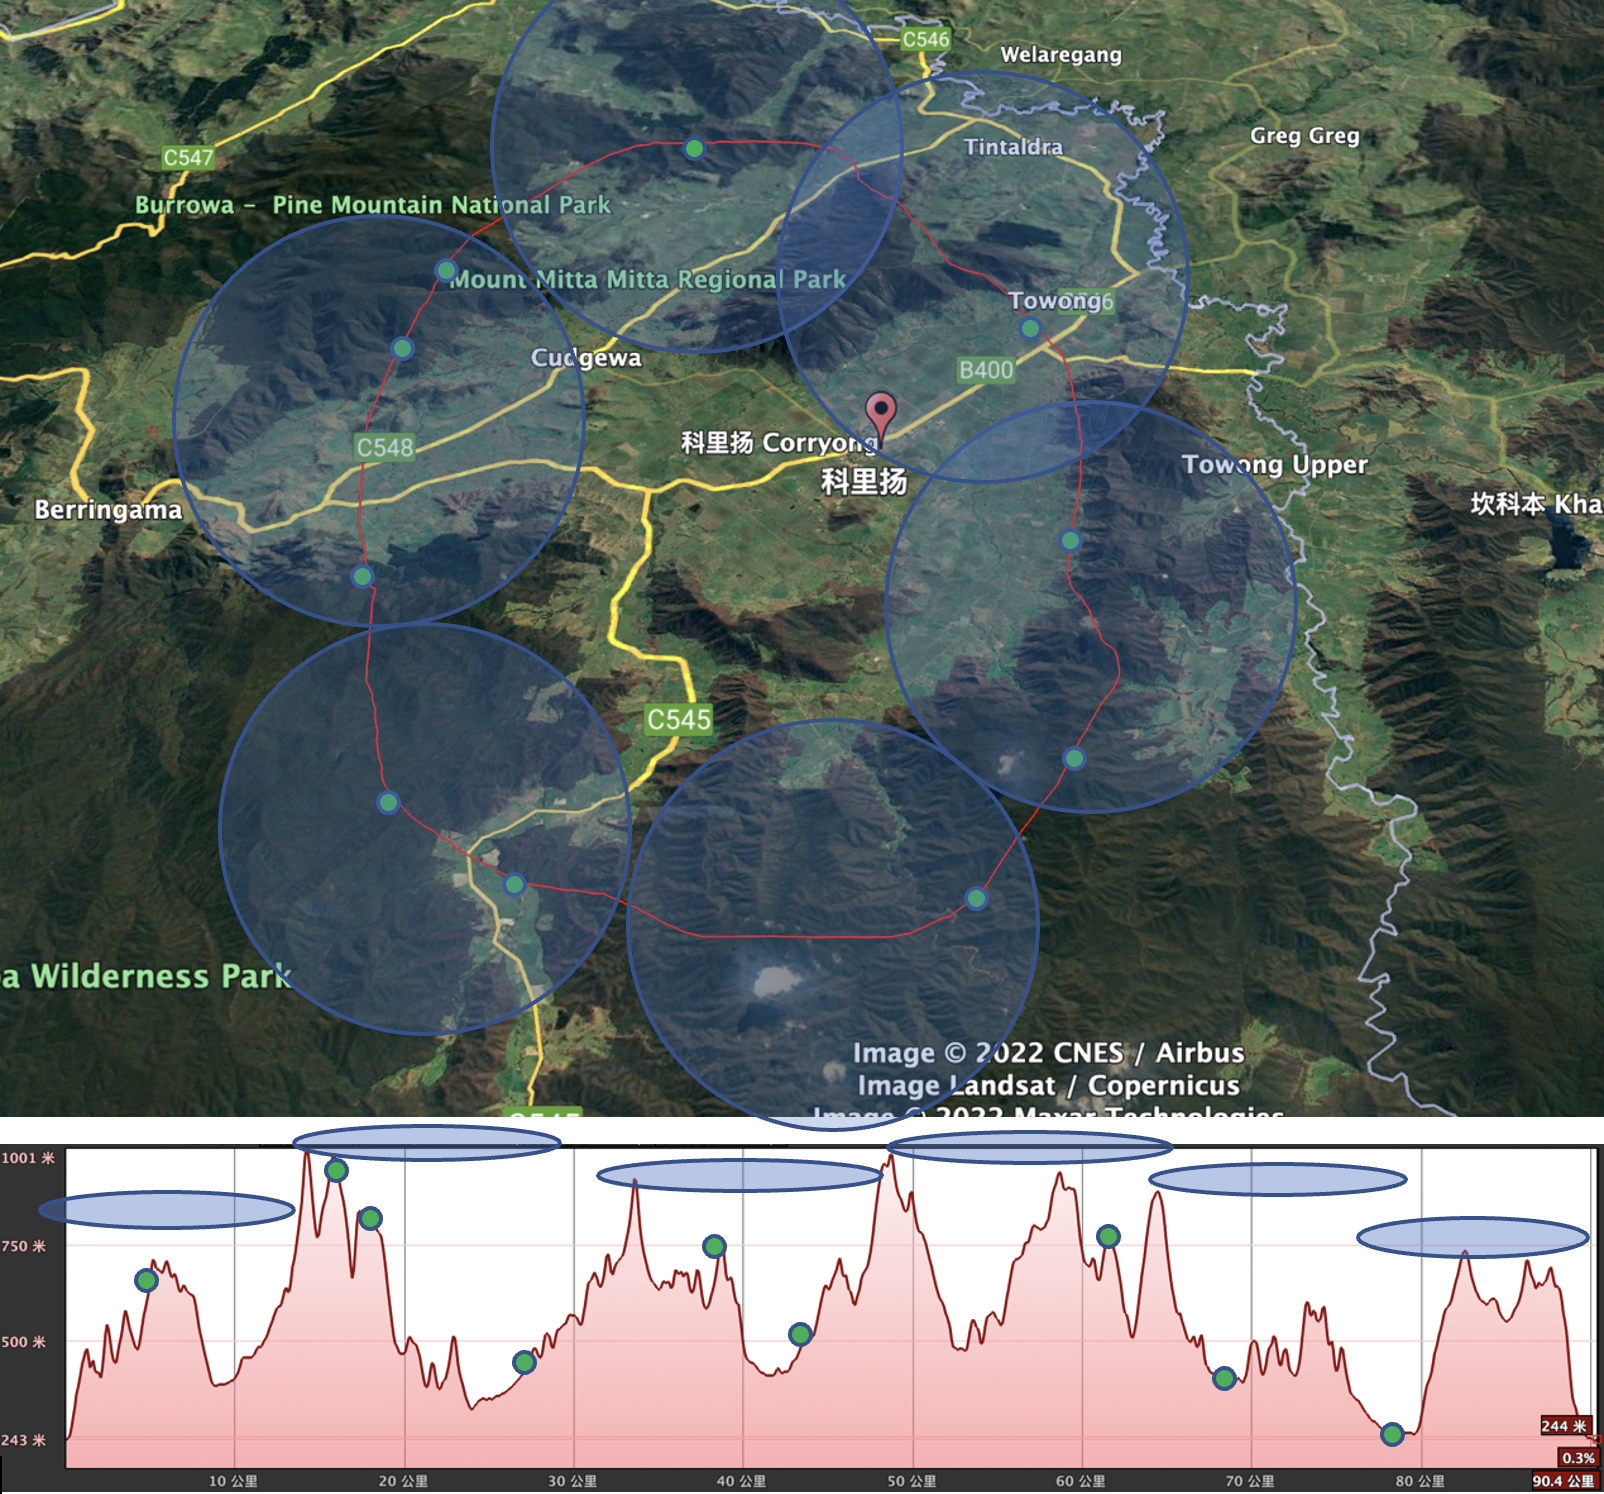
\includegraphics[width=.7\linewidth]{drones.png}
      \caption{Simulated distribution of drones \\ Blue circles show the radio range of the transceivers on the
drones}
      \end{figure}
      
Blue circles and lines show the radio range of the transceivers on the
drones

Drones' location strategy common derivation

Above is a specific situation of the distribution of the drones, in more
common situations, the distribution of drones is related to the terrain
and distribution of the fire fighters.


\end{document}
